\documentclass[11pt,twoside,letterpaper]{book}

\def\theshorttitle {UVa HSPC Guide}
\def\thelongtitle {University of Virginia High School Programming Contest Guide}
\title {\thetitle}
\author{Association for Computing Machinery Student Chapter at the University of Virginia}

% Packages
\usepackage{wrapfig}
\usepackage{epsfig}
\usepackage{fullpage}
\usepackage[letterpaper,centering]{geometry}
\usepackage{fancyhdr}
\usepackage{lastpage}
\usepackage{enumitem}
\usepackage{ifthen}
\usepackage{palatino}
\usepackage{hyperref}
\usepackage{float}

% Page offsets
\setlength{\topmargin}{-.5in}
\setlength{\oddsidemargin}{-0.25in}
\setlength{\evensidemargin}{-0.25in}
\setlength{\textwidth}{7truein}
\setlength{\textheight}{9truein}
\setlength{\parskip}{6pt}
\setlength{\hoffset}{0in}
\setlength{\voffset}{-0.2in}
\setlength{\headheight}{0.33in}
\setlength{\headsep}{0.5in}
\setlength{\marginparwidth}{0in}

% Page Numbering as 1, 2, 3, etc
\pagenumbering{arabic}
\pagestyle{fancy}

\newcommand{\footurl}[1]{\footnote{\scriptsize\url{#1}}}

% adapted from https://tex.stackexchange.com/questions/121865/nameref-how-to-display-section-name-and-its-number?rq=1
\newcommand*{\fullref}[1]{\hyperref[{#1}]{\autoref*{#1}: \nameref*{#1}}}

\cfoot{\theshorttitle}
\rfoot{\thepage\ of \pageref{LastPage}}

\providecommand{\tightlist}{%
  \setlength{\itemsep}{0pt}\setlength{\parskip}{0pt}}

\newenvironment{itemlist}{
\begin{itemize}
\setlength{\itemsep}{0pt}
\setlength{\parskip}{0pt}}
{\end{itemize}}

\begin{document}

\title {\huge High School Programming Contest Guide \\
\vspace{1in}
\resizebox{3in}{!}{
\includegraphics{images/icpc-hspc-logo.png}}
\vspace{1in}
}
\author {\Large Compiled by ACM @ UVa}
\maketitle

\cleardoublepage

\tableofcontents

%----------------------------------------------------------------------
\cleardoublepage
\chapter{Introduction}

Put intro here\ldots

This guide is the result of efforts by a number of individuals at the
University of Virginia.  We have hosted high school programming
contests since 2011, and started collecting our notes shortly
afterward.  This document evolved over the next few years, and was
written in this for for the ``Organizing a High School Programming
Contest'' workshop at SIGCSE
2018\footurl{https://sigcse2018.sigcse.org/attendees/workshops.html}.
The latest version is available online at
\url{http://aaronbloomfield.github.io/hspc}, which is sourced from a
Github repository at \url{https://github.com/aaronbloomfield/hspc}.


\section{Licensing}

This document, and the rest of the materials contained therein~--
except for the logo~-- are released under a Creative Commons
Attribution-ShareAlike 4.0 International
License\footurl{https://creativecommons.org/licenses/by-sa/4.0/} (CC
BY-SA).

The following HSPC logo is used throughout this document:

\begin{center}
  \resizebox{2in}{!}{
\includegraphics{images/icpc-hspc-logo.png}}
\end{center}

This logo was derived, with permission, from the main ICPC logo, which
can be found online at the ICPC
website\footurl{https://icpc.baylor.edu/}.  The logo is owned by the
ICPC Foundation, and they have given permission for high school
contests to use the system if\ldots



%----------------------------------------------------------------------
\cleardoublepage
\chapter{Preparation}

\section{Early Planning}

All of these should be done around 6 months before the date of the
contest itself.


\subsection*{Who is going to run the contest?}

Determining who is going to run the contest is the very first step.
Different institutions use different models.  At UVa, it is primarily
run by the students in our local ACM chapter, with assistance from a
faculty advisor.  The University of Maryland, which has run a very
popular contest every year since at least 1998, has much more of the
organization run by the department (faculty and/or staff).  Obtaining
administrative support from your department for various tasks will be
quite helpful.

For the contest itself, there are two primary roles that need to be
defined.  One is the Contest Director, who is the person coordinating
the majority of the contest.  The Head Judge (or Chief Judge) is the
individual responsible for coordinating the problem generation, and
managing the judging at the contest itself.


\subsection*{What computers will be used?}

Different contests will use different computer setups.  Part of this
step will be to decide the team size (see below).

We have used computer labs at UVa for our contests.  This allowed
students to have a full sized monitor, as well as a keyboard and a
mouse.  We used a VirtualBox environment (described later in this
document) for their environment.  The drawback to this model is that
the capacity is dependent on the number of computers and computer
labs~-- and if they are spread throughout your institution's campus,
then there is more travel time to the contest sites.  At UVa, we used
5 labs that can hold 49 people each (as per the fire marshal's limits)
-- however, one of them only has 7 usable computers due to the lab
layout.  This allowed a total of 55 teams (12 in the four larger labs,
7 in the smaller one), which was our registration cap.  Many
college-level ICPC contests use this method.

Many schools will use laptops for each team -- the University of
Maryland has used this very successfully.  The challenge to this is
where to securely store the laptops between contests.  Purchase and/or
support of the laptops is another support issue.  The laptop screens
are typically smaller than a monitor screen, which makes it more
difficult for a four person team to use it effectively.  Advantages
are that one can still load up a custom environment on the machines,
which we found very necessary (see later in this document for
details).  Furthermore, there are many more lecture rooms that can
accommodate students with laptops, as one does not require a lab with
pre-installed computers.  One can supply keyboards, monitors, and mice
along with the laptops, although this will add to both the cost and
storage issue.

One could require the students to bring their own computers.  This is
easiest to support, but it is difficult to enforce a custom
environment.  A very common aspect of the contests is to eliminate
Internet access (except to the submission server) during the contest
itself.  We do this through the setup on our VirtualBox image.  This
is more difficult when the machines are not managed by the host
institution.  We realize that one can exit a VirtualBox image on any
machine, but this has not yet been a problem.  One could distribute a
VirtualBox image, and require each participating team to have
VirtualBox installed prior to the contest.

Lastly, one can adopt a hybrid approach.  For UVa's 2018 HSPC, we have
70-80 teams that are interested, and only 55 spots in the computer
labs.  We are currently investigating using UVa supplied laptops in a
lecture hall to allow more participants to participate.  In future
years (2019 and beyond), we are hoping to obtain funding to buy a set
of laptops (along with monitors, keyboards, and mice) specifically for
this purpose.


\subsection*{Understand the financial costs}

The contest will cost some amount of money: food, prizes, t-shirts,
etc., all will have some expense.  Some of these can be lowered or
eliminated (no t-shirts, for example), or paid for by other entities
(the school or department).  A 50 team contest at UVa typically costs
around \$7,000 to run~-- the budget section is included later in this
document.

Team registrations are one way to pay for this.  However, having too
high of a registration cost will deter schools from participating.
For our contests, that would mean about \$150 per team to register.
High schools often do not have the budget to spend \$450 to send three
teams.  Thus, we sent the cost at \$40 per team, as this seemed like
an affordable expense.  The registration cost from the teams only paid
for the t-shirts.  This meant, however, that we had to raise about
\$5,000 to allow the contest to run.


\subsection*{Set reasonable expectations}

Our first contest, in 2011, had a total of three teams.  It was a huge
amount of work, as we had never done this before.  But the contest
only grew in size, and we now have to turn teams away, as we typically
reach our room capacity (ways to mitigate that are explained in this
document).  However, we all had a great time with the contest, and we
had more teams in successive years (17 in 2012, 34 in 2013, and
we hit our cap of 50 teams in 2014 and every year since).


\subsection*{Generate a list of all high schools to be invited}

As the contest becomes more well known, this becomes easier, as the
schools will find you.  However, when starting the contest from
scratch, one will need to generate a list of emails to be sent.

We defined the target area that we were expecting to attract students
-- since we are located in central Virginia, we defined the entire
state of Virginia as that target area.  For a high school running such
a contest, it may be that the high schools in the local area are the
extent of the target area.

We looked up each high school therein, and found an email address for
each school.  We attempted to get the email address for a computer
science teacher at the school -- often this was not available online,
so one could call the high school to ask who the computer science
teacher was.  If there was no obvious contact, we would ask for the
best person to send the information to.  The task of finding was split
among multiple student volunteers, as there are over 300 high schools
in Virginia.

Another option would be to leverage affordable services from
Amazon Mechanical Turk, although we did not pursue this option.

We kept this information, as we used the list in future years.
Creating an appropriate HSPC announcement mailing list for your
institution is another possibility.  Often we would receive a
response that they are forwarding it to a more appropriate person, so
we updated the list appropriately.


\subsection*{Decide if it is going to piggyback on another event}

One option is to have it be the same date as an on-campus event~-- for
many years, we did this with the Engineering Open House (a day where
accepted or interested students can take a tour of our Engineering
school and facilities).  This has the benefit of bringing in many high
school students interested in computing to the open house.  They are
typically coming from far away, and are often interested in attending
both events.  The disadvantage is that scheduling rooms is very
difficult, as all the other participants in the other event will want
the same rooms.  As our contest grew in size, and we needed more rooms
to accommodate the participants, we ran into too many scheduling
problems when it was the same date, and we have since moved it to a
different weekend.  However, this worked very well when our contest
was small.


\subsection*{Pick a date}

If the date is not decided upon by the above step, then this is far
more difficult than it sounds.  It can't be too close to the AP exams.
The date needs to avoid other contests, such as robotics tournaments
(as many students are active in both robotics and programming
contests).  It will need to avoid high school spring breaks and prom
season. In order to recruit a sufficient number of volunteers to help,
we had to avoid UVa's spring break (both he start weekend and the end
weekend as well).

Because UVa is active in the collegiate level ICPC, we would hold our
HSPC in the spring (in March or April); other schools hold theirs
throughout the year.  Some years there were few options due to the
constraints above.  After our participation rate increased, we would
email the coaches from last year a request to fill out a quick Google
Forms survey as to what weekends worked the best.  For us, most high
schools seemed to be on a somewhat similar schedule, so this greatly
aided us to find a date.


\subsection*{Reserve rooms}

This is critical, as you can't have a programming contest if you don't
have the computer labs, auditorium, etc.  Make sure that, if it is on
the date of another event, that those from the other event will not
try to take your rooms away from you. We were always sure to reserve
our rooms prior to opening up the registration, for obvious reasons.
On some years, other events would suddenly ``need'' those rooms on
that date, but as they did not reserve them ahead of time, we were
still able to use them.


\subsection*{Start generating problems}

Good quality programming contest problems take many, many, MANY
iterations to get right.  Getting the difficulty level correct is the
biggest challenge.  people generate multiple problems, and then let
the group pare down the selection from there.  See the Problem
Generation section, below.


\subsection*{Start advertising}

Email all the coaches, post on social media, and on the departmental
website.  Emailing the coaches from previous years helped as well.  We
would generate a Twitter hash tag (we would use \#uvahspc2017), and
promote it there.  Be sure to state the registration cost when
advertising.


\subsection*{Open up registration}

We discuss online registration systems elsewhere.  A custom system
works great, but can be a chore to maintain.  One can also use various
Google Forms to handle registration.  The first one would be for a
school to state how many teams.  Other forms can follow (team members,
food allergy information, etc.).  Be sure to include payment
information (amount and how to pay) along with the registration.


\section{Schedule}

It will be easiest on the participating schools if the schedule is
known during registration, as the schools will have to arrange
transportation.  Many of our schools would drive from 2 hours away
(the time taken to drive from northern Virginia to Charlottesville),
so we could not start the contest too early.

Here is a typical schedule:

\begin{itemlist}
  \item 8:30 a.m.\ --\ 9:30 a.m.: Registration (with some type of
    breakfast)
  \item 9:30 a.m.\ --\ 10:30 a.m.: Opening talk and rules
  \item 10:30 a.m.\ --\ 11:30 p.m.: Practice contest (includes time to
    travel to and from)
  \item 11:30 p.m.\ --\ 12:30 p.m.: Lunch
  \item 12:30 p.m.\ --\ 4:30 p.m.: Actual contest
  \item 4:30 p.m.\ --\ 5:00 p.m.: Close-down time (travel to the
    closing talk, etc.)
  \item 5:00 p.m.\ --\ 5:30 p.m.: Closing talk
\end{itemlist}

\noindent A number of things to keep in mind:

\begin{itemlist}
  \item We have often tweaked the schedule after registration, but we
    have never modified the starting time from what was first stated
    during registration, as that would have required a change to the
    schools' transportation plans.
  \item The contest length itself is the most important aspect, as
    that will determine the overall schedule.  We have found a four
    hour contest to be about right for high school students, but
    different contests will have different lengths.
  \item There will be time needed for the participants to move from
    one location to the other, so that should be considered when
    determining the schedule.
\end{itemlist}


%----------------------------------------------------------------------
\cleardoublepage
\chapter{Problem Creation}

Problem generation has been one of our biggest challenges.  From a
collegiate perspective -- both faculty and students -- it is difficult
to understand the level of knowledge of high school students.  If the
problems are too hard, then some teams will not solve any, which can
be dispiriting.  If they are too easy, then some teams will finish
early, which is less than ideal.

\section{Background}

Include info here from Blythe's presentation about what high school
students know (based on their classes).


\section{Problem Difficulty}

Include info here from Blythe's presentation about the beginner /
experienced / advanced difficulty levels, and how to have a good
``slope'' of problems.

In 2012, there were probably too many easy problems. Consider having a
few more medium problems and a few less easy ones. Also, the
contestants found problems involving numbers much easier than anything
that involved string parsing, so consider making the easiest few
problems involve simple math operations.

In the 2011 contest, there were eight problems that spanned the easier
half of ICPC regional problems. These problems were almost universally
viewed as too difficult. The 2012 featured ten problems, containing 5
problems on par with the easiest problem at an ICPC regional, two
medium-level problems, and three hard problems. The medium problems
were still probably on the easier side by ICPC standards; the hard
problems were much more typical ICPC problems.  These problems were
much better received, although there were a few complaints about the
jump between the easy and medium problems and that there were not
enough problems that required the teams to think.

\section{Development}

Our problem development would start early~-- ideally 6 months prior to
the contest, although we did not always achieve this.  The problems
progressed through many different stages of development.  The first
step was general brainstorming; a one or two sentence description of a
potential problem, categorized by difficulty and problem type. About
four times the necessary problems should be created using this method,
so that culling can occur very easily. It is very important not to get
attached to a particular problem at this point; if the problem is
confusing or overly difficult it should not end up in the final
problem set.

From there, we selected roughly 15 problems to investigate further and
write up full problem descriptions for them. One very useful thing
that was done in the past was ensuring that for the first few
iterations, only a few people had read each problem. This ensured that
at the later stages, a fresh pair of eyes looked at the problems
without bias and inherent knowledge of the problems. At this point,
there should be a pretty clear indication of which problems are worth
pursuing.

Next was to assemble the packet of problems and proofreading the
packet.  Again, try to get a new set of eyes to look over each
problem. Try to get at least three distinct solutions to each problem;
one would be surprised how many bugs appear when different people
write solutions. Specifically, each problem should be solved at least
once in each contest language.  A few times when we did not do this,
we ran into problems: in 2012, we could that C++ handles floats
differently relative to the other languages (even though we had a
validator for that problem!), and in 2014, we found that C++ handled
longs differently relative to the other languages.  Consider having
your solution throw an Exception when illegal input is passed in
(meaning, a negative number is passed when only positive numbers are
allowed). This will help detect errors in the input generation code.

Problems should be 100\% complete more than a week before the
contest. There are far too many other things to do right before the
contest to be worrying about the specifics of the problems.


\section{Input and output considerations}
\label{sec:input-types}

Program input should be as easy to parse as possible, as this will
allow the students to focus on the problem solving, and not input
parsing.  Similarly for the output format.

Any problem will be tested against multiple test cases.  Some contest
submission systems will have all the test cases in one file, and the
program will run once, and then determine the out for all of the test
cases.  PC$^2$ traditionally uses this format.  Other submission
systems will have many different input files, one test case each, and
the program will be run multiple times~-- once for each test case.
Kattis uses this format, and PC$^2$ has started using it recently as
well.  Which system you use will determine some of the input and
output specifications.

Older ICPC problems would read in test cases until the end of input~--
however, finding the end of the input stream always took a bit longer
to code, and we have found that to be more difficult for some of the
beginner high school students.  Many recent problems will always start
with a single integer on the first line of the input file which is the
number of test cases, and then each test case will have a specific
format.  If there are multiple ``things'' that a test case has (such
as multiple nodes in a graph path problem), then having a single
integer preceeding the list of nodes will help input parsing.

Whitespace in output can be a problem.  If the output requires a list
of integers on online, space separated, then is a space at the end of
the line allowed?  Having said space is easier to implement (in the
{\tt for} loop that prints the output, just print out the value
followed by the space) rather than not allowing it (in the {\tt for}
loop that prints the output, one has to put a test to see if it is the
last value to be printed on the line).  Having very strict
requirements for the output format will disadvantage less experienced
teams, as they will not be as familiar with these details.  Submission
systems can ignore whitespace, although some of them will ignore {\em
  all} whitespace on a line, which may not be desired (as ``1 2 3''
will then be the same as ``123'').  Often the required output format
can be changed to require one value per line, which is easier to both
output and to verify.

Input that can be easily read in without dealing with whitespace makes
it much easier to parse.  Students will tyipcally use a input means
that ignores whitespace ({\tt Scanner} in Java, {\tt cin} in C++,
etc.).  An input file that is just a series of numbers will be easiest
to handle, as the whitespace between them will be ignored by these
routines.  Reading in a string that can contain whitespace will be
very difficult -- but a string that has no whitespace is also easy for
them to handle.

Problems with multiple correct answers will require a validator
program; these are described below.

We would often create an input generator that would create a large
input file.  This should test most corner cases, but feel free to add
in additional cases as well.  We would add to this certain cases
(corner cases, empty cases, etc.) to generate the full judging input.
Ensure that the judging data takes no more than 20 seconds to run on
any of the solutions, as this gives a reasonable timeout level to test
against.

Having all of the problems use the same input and output specification
(having ``Case x:" before each solution, etc.) was exceptionally
helpful. It allowed teams to figure out how to specify output in the
practice contest and then use what they learned in the actual contest.
It also allowed us to be more consistent when generating the sample
and judging output.


\section{Theming}

Starting in 2014, we started theming our problems -- we would rephrase
the ``plot'' of the problems so that they all followed a theme.  This
certainly wasn't necessary, but we felt it made the contest more
enjoyable.  The themes we have used:

\begin{itemlist}
\item 2014: Lord of the Rings
\item 2015: Avengers (the movie had recently come out)
\item 2016: Breakfast
\item 2017: Classic Nintendo Games
\item 2018: Pixar movies
\end{itemlist}

For more difficult problems, we found it was easier to generate the
problem first, and then apply a theme to it.  For the less difficult
problems, we found it easier to pick a theme (Pixar movie, breakfast
food, etc.) and then create a simple problem based on that idea.


\section{Validators}
\label{CustomValidators}

A validator is necessary when a problem has more than one correct
answer.

One example of this is a problem whose answer is a floating point
number -- rounding errors or differing precision can cause values to
vary slightly in the less significant digits.

Some contests will
require the answers be a fixed precision.  For high school contests,
we feel that this causes them to focus a lot of their time and effort
on the exact formatting of the output, rather than the problem
solving.  There are also rounding differences between the programming
languages, which will cause a language-dependent difference.  As an
aside, did you know that there are five different standards for how to
round
numbers\footurl{https://en.wikipedia.org/wiki/IEEE_754\#Rounding_rules}?

Other examples include finding a path through a maze or other graph
(as there may be multiple paths), or finding the order to do a set of
tasks (some items can be done in either order).

If there is only one correct answer, then the correctness of the
solution can be checked via file comparison with the correct solution.
The submission systems, discussed later, have the ability to ignore
whitespace when performing said comparison.

If a problem has multiple correct answers, then a {\em validator} -- a
program that reads in the solution and returns whether it is a correct
solution or not -- will have to be written for that problem.

{\bf We do not recommend using validators!} At least not until one is
familiar with the contest submission system.  It is often the case
that a problem can be rephrased so that there is only one correct
solution.  A validator takes a fair amount of time to write and test,
especially during the busy time of contest preparation.  If the
validator does not work properly during the contest, then the contest
judges will have to manually judge each answer.

Recent contests at the collegiate ICPC level, have generally avoided
problems that require validators.  UVa's HSPC has generally avoided
them as well~-- we tried using a few in 2012, and didn't like the
experience, and have avoided it ever since.

The format for custom validators will vary based on the contest
submission system used.

The high-level overview of validators is that the program will read in
the problem input and the submission solution that was generated.
There are two methods for writing effective validators; one is having
essentially a solution embedded within the validator which calculates
the result and then compares it with the returned result.  This is
useful for floating point results, as one can compare within a certain
accuracy (say, $10^{-5}$).  The other is that the validator will have
to trace through the provided solution to see if it really does solve
the problem.  This is necessary for solutions that can have different
paths.


%----------------------------------------------------------------------
\cleardoublepage
\chapter{Configuration}

\section{System Configuration}

We have tried using multiple configurations for our contests.
Initially our system support staff allowed us to customize the
environment in the labs.  As the number of teams grew, and we were no
longer able to fit in one lab, this became impractical.  Next we tried
using USB keys to boot to a customized version of Linux for a few
years, but found the USB key reliability -- as well as speed -- to be
difficult to make that work.  Furthermore, replicating the keys took a
lot of time.

As of the 2015 contest, we are now using a VirtualBox image.  The
instructions for setting up this image can now be found in
\fullref{appendix:vb-image}.  They are based on the directions that
can be found
online\footurl{http://aaronbloomfield.github.io/slp/docs/virtualbox-image-details.html}.


\section{Submission systems}

There are multiple submission systems available.  We have used PC$^2$,
as one can easily download it and install it on an institution's own
servers.  We discuss three submission systems here.

\subsubsection{PC$^2$}

PC$^2$ stands for Program Contest Control, and is a widely used
system.  It is written in Java, and is still being updated.  It can be
downloaded for free online\footurl{https://pc2.ecs.csus.edu/}.  Its
usage is described in detail in \fullref{appendix:pc2-config}.

\noindent{Pros:}

\begin{itemize}
  \tightlist
\item This system is free to use, and can be run on one's own servers.
\item It is widely used, and has a lot of documentation available.
\item This usually uses the input format of all test cases in one
  input file (see \ref{sec:input-types}).  If a problem is online in
  the other format (one test case per input file), it can easily be
  converted to all be in one file (just put a integer number at the
  top with the number of test cases therein).
\end{itemize}

\noindent{Cons:}

\begin{itemize}
  \tightlist
\item The system is often buggy, and we had the entire judging system
  be so buggy that it was unusable because of this.  Other features
  (such as problem copy) do not work, but this is not always evident
  until much later.
  \item It is not open source, which makes it very difficult to figure
    out what is going wrong, much less to fix it.
\end{itemize}

\noindent{Warnings:}

\begin{itemize}
  \tightlist
\item There is a separate connector program available, which allows
    for the submission (and judging) to happen through a web-based
    interface.  However, this connector has some {\bf SERIOUS} issues
    -- it forks off a thread for {\em each} connection (team, judge,
    etc.).  However, most apache2 installations have a default limit
    of 50 threads, which can easily be reached by the connector.  The
    mid-Atlantic ICPC regional contest in 2016 was a disaster because
    of this~-- with over 200 connections, nobody was able to connect
    for hours after the contest started.
\end{itemize}


\subsubsection{KATTIS}

KATTIS\footurl{https://open.kattis.com/} is an online system
originally developed by KTH Royal Institute of Technology in
Stockholm\footurl{https://www.kth.se/en}.  It is now its own entity.
It is described in detail at \ldots

\noindent{Pros:}

\begin{itemize}
  \tightlist
\item This is, by far, the most refined system available.  It has been
  used in multiple ICPC world finals for this reason.
\end{itemize}

\noindent{Cons:}

\begin{itemize}
  \tightlist
\item One cannot run this on one's own servers, which means that one
    will have to provide an open Internet connection to the kattis
    servers -- which also means that contestants can view other
    problems and solutions.
\item Because one cannot run this on one's own servers, one will
    have to get KATTIS to setup and configure the contest.  It is
    unclear if they would be willing or able to do this for high
    school contests.
  \item This usually uses the input format of one test case per input
    file file (see \ref{sec:input-types}).  If a problem is online in
    the other format (all test cases in one input file), it is more
    difficult to convert in this direction.
\end{itemize}

\noindent{Warnings:}

\begin{itemize}
  \tightlist
\item As mentioned above, one has to get the assistance of the KATTIS
  staff to setup and configure a contest.
  \end{itemize}


\subsubsection{DOMjudge}

DOMjudge\footurl{https://www.domjudge.org/} is a free and open source
web-based submission system.  Its usage is described in detail in
\ldots

\noindent{Pros:}

\begin{itemize}
  \tightlist
\item This system is free to use, and can be run on one's own servers.
\item It is open source, so modifications or bug fixes can be
  contributed by many individuals
\end{itemize}

\noindent{Cons:}

\begin{itemize}
  \tightlist
\item \ldots
\end{itemize}

\noindent{Warnings:}

\begin{itemize}
  \tightlist
\item \ldots
\end{itemize}




%----------------------------------------------------------------------
\chapter{Preparation Todo Lists}

\section{Previous semester}

\begin{itemlist}
\item Reserve rooms, set date, open registration
\end{itemlist}


\section{2 months out\ldots}

\begin{itemlist}
\item Get t-shirt artwork
\end{itemlist}


\section{1 month out\ldots}

\begin{itemlist}
\item Photo release form for minors\ldots
\item Close registration
\item Order UVa catering lunch
\item Order t-shirts
\item Order coach gifts (mugs)
\item Order prizes, certificate paper, name badges, holders, and
  lanyards, balloons (if needed), balloon ribbon
\item Arrange for the media to show up!  Contacts:
  \begin{itemlist}
    \item Derek Quizon (dquizon@dailyprogress.com) at the Daily
      Progress
    \item \ldots
  \end{itemlist}
\end{itemlist}


\section{Week-of checklist}

\begin{itemlist}
\item Acquire coach gifts and t-shirts
\item Communicate with admissions, if they are going to show up
\item PC$^2$ configuration; also plan for backup servers if the main
  PC$^2$ server dies.
\item Final email(s) to coaches: parking information, finalize the
  team member names (and team names!), get t-shirt sizes for
  chaperones
\item Poster (ideally in a holder) for outside the initial meeting
  building
\item Reserve balloon helium
\item Server account setup (the Linux login setup, not PC$^2$
  configuration).  Also plan for backup servers (backing up of
  accounts).
\item Contestant web site setup: this is the website that contains the
  following types of links: cheat sheets, scoreboard link, Java API,
  sample input and output, problems PDF, etc.  Ideally, this will be
  the browser's default home page.
\item Email reminder to teams that have not paid
\item Public website setup; this includes the scoreboard
\item Reserve Bodo's
\item Buy stuff from Costco: candy, bottled water, soda, coffee stuff,
  etc.
\item Coordinate volunteers, along with roles (judge, etc.) (who,
  when, how); likely at a volunteer meeting
\item Create floor plan of the competition
\end{itemlist}


\section{Day before checklist}

\begin{itemlist}
\item Name tags: print them, put them in the badge holders, attach
  lanyards
\item Pick up helium tank
\item Prepare contest presentations, for both the welcome ceremony and
  the conclusion ceremony
\item Set up print system
\item Pick up Bodo's
\item Creation of the registration packets. Put it in a nice folder,
  and include various things: schedule, information about UVa and the
  CS program, \ldots
\item Copying of problem packets
\item Prep the explanation of all the questions, including slides;
  this is in the closing ceremony.
\item Webcams if there is time: this allows the coaches to see their
  teams competing.
\item Printing of the certificates
\item {\bf SYSTEM TEST!!!!}
\item Create signs for the day of the contest (this way to the
  computer labs, that way to the auditorium, etc.)
\item Detailed script for the intro presentation and the awards
  ceremony, including who is saying what
\end{itemlist}  

\section{Day of checklist}

\begin{itemlist}
\item Printing of packets (all)
\end{itemlist}

%----------------------------------------------------------------------
\chapter{Contest Logistics}

\section{Other notes to file somewhere\ldots}

This is a section for notes that need to go somewhere, but where that
somewhere is has not yet been determined.  This section is not
expected to be in the final version of this HSPC guide.

\begin{itemize}
\item For the nametags, print out two of each nametag, and have them
  facing out in both directions.  This way, when the name tag gets
  flipped around, you can still see who that person is.
\end{itemize}

\section{Roles}

After the 2013 HSPC, when we had 39 teams, and over 150 students, we
had the realization that we would need different roles that volunteers
could fill, and a set of responsibilities for those roles.  The
responsibilities are split into two parts: preparation for the
contest, and during the contest.

Many of the tasks that are listed in these roles start with 'ensure',
as it is not necessarily the person in that role who will be doing the
task.  But it is the person in that role who will be ensuring that the
task is completed successfully.

Unless listed otherwise, most roles only require one person.

\subsection{Head Judge}

\noindent Before the contest day:

\begin{itemlist}
\item Ensure that all the contest judges have a computer that can boot
  up Linux, and that they can connect with PC$^2$
\item Ensure that the judges are assigned to the problem(s) they will
  judge, and that they are very familiar with those problems
\item Ensure that s/he is familiar with ALL the problems
\end{itemlist}

\noindent Contest day:

\begin{itemlist}
\item Prior to both the practice and actual contest, ensure that the
  judges are all in the judging room and logged into PC$^2$ when the
  practice or contest is about to begin
\end{itemlist}


\subsection{Contest Judge}

\noindent There will be multiple contest judges, with each one judging
a small number of problems (1-3).

\noindent Before the contest day:

\begin{itemlist}
\item Ensure that s/he has a working Linux system, with PC$^2$
installed and configured
\item Once the judging problem assignments are assigned, familiarize
  himself/herself with the problems
\item Ensure that they know how to use pc2judge
\end{itemlist}

\noindent Contest day:

\begin{itemlist}
\item Arrive at the judging room well prior to the start of the
  practice / contest
\item Judge the problems!
\end{itemlist}


\subsection{Site Director}

\noindent There is one site director for each site that the contest is
being held at.  Neighboring classrooms are considered one site, but
classrooms in different buildings are different sites.  The site
director is expected to stay on--site during the practice and contest.

\noindent Before the contest day:

\begin{itemlist}
\item Ensure that the computer configuration is all ready to go.  The
  site director is not in charge of the configuration itself, but s/he
  will need to know how to boot up the machines, solve problems, etc.
\item Ensure that the team mappings are known (each team has a
  location in the room, a team number in PC$^2$, and a computer
  number; this needs to be able to be quickly mapped during the
  contest, and this will also be needed by the balloon manager)
\item Ensure that lines of communication with the contest director
  (and others) are known: cell numbers, etc.
\end{itemlist}

\noindent Contest day:

\begin{itemlist}
\item Ensure all the machines are booted into the contest environment
  well before both the practice and contest starts.
\item Ensure that the home directories are wiped (before both the
  practice and the contest)
\item Ensure that printing works, and that the printer is all
  configured and ready to go
\item Supervise the volunteers who are acting as monitors
\item Communicate with the person managing the balloons to make sure
  that they have everything they need (management of the balloons is a
  different role; but that role and the site director will need to
  communicate)
\end{itemlist}


\subsection{Balloon Manager}

\noindent There is one balloon manager, who will supervise the balloon
distributors at the various sites.  Note that balloons are typically
not distributed during the practice contest.

\noindent Before the contest day:

\begin{itemlist}
\item Ensure that there are enough balloons, of the appropriate
  colors, to distribute to all the teams
\item Ensure that the ribbon is ordered, and that scissors are ready
  for each site
\item Ensure that the helium tank(s) is/are ordered; one tank will be
  needed for each site; alternatively, if helium is not being used,
  then ensure that whatever balloon display method is ready to go
\item Ensure that the PC$^2$ judge logins are ready for each site, as
  the people distributing the balloons will need to be logged into
  PC$^2$ to determine which balloons to distribute
\item Ensure that each site has a Linux machine available for logging
  into pc2judge
\item Know how to configure PC$^2$ for balloon distribution (see
  section~\ref{sec:pc2judge-balloons})
\item Ensure that the balloon distributors are trained how to read
  pc2judge and distribute the balloons.  This is essential.
\item Ensure that the site mappings (done by each site director) are
  known and available during the contest
\end{itemlist}

\noindent Contest day:

\begin{itemlist}
\item Ensure that every site is ready to go for the balloon
  distribution for the contest
\item Ensure that the balloon pc2judge accounts are logged in at each
  site
\item Supervise the volunteers distributing the balloons
\end{itemlist}


\subsection{Food Tzar}

There are three food meals that need to be ordered for the contest:
a light breakfast, lunch, and snacks/drinks during the contest.

\noindent Before the contest day:

\begin{itemlist}
\item Ensure that each of the three food meals have been ordered
\item Check the rules at each site as to what food is allowed at which
  site; all sites must have the same types of food available
\item Ensure that the various special food considerations (vegan,
  vegetarian, allergies, gluten-free) are handled
\item In the event that we're dealing with UVA dining, make clear to
  them that you are the person they should contact when food arrives,
  and make this clear to the other volunteers as well.
\end{itemlist}

\noindent Contest day:

\begin{itemlist}
\item Manage the acquisition and/or delivery of that food; in
  particular, be there to receive the catering, if that is how lunch
  is arriving
\item Ensure that clean-up is handled properly (grab volunteers that
  day for this)
\item Ensure that the various special food considerations (vegan,
  vegetarian, allergies, gluten-free) are handled
\end{itemlist}


\subsection{System Administrator}

\noindent The list below assumes that the computers in the contest are
going to be booted off of a USB key.

\noindent Before the contest day:

\begin{itemlist}
\item Ensure that enough USB keys are available
\item Oversee the configuration of the Linux image used during the
  contest
\item Oversee the backup system of the contestant's home directories
  to the appropriate backup sever
\item And be sure to know how to restore from a backup image
\item Ensure that all the USB keys are properly duplicated
\item Ensure that the printing system is working and ready to go
\item Coordinate with the faculty advisor to ensure that the computers
  being used can be booted up on the USB keys, and that printers are
  available (one per site, with extra paper and toner cartridges)
\item Test the system prior to the contest
\end{itemlist}

\noindent Contest day:

\begin{itemlist}
\item Help the site directors with the booting up of the computers via
  the USB keys
\item Ensure that the printing is working
\item Be available to solve any system-related issues
\end{itemlist}


\subsection{Coach Liason}

\noindent Before the contest day:

\begin{itemlist}
\item Obtain guest wireless access codes for the coaches (from
  \url{https://network-setup.itc.virginia.edu/}, click on ``generate
  wireless passcodes''.  In the right-hand box (labeled ``need a lot
  of passcodes''), click ``advanced guest wireless passcode
  generation'', and fill out the form.
\end{itemlist}

\noindent Contest day:

\begin{itemlist}
\item Ensure that a volunteer is sitting in the coach room during the
  practice and the contest; this need not be the coach liason
  himself/herself
\item Check in on the coaches from time to time during the practice
  and contest
\end{itemlist}


\subsection{Volunteer Coordinator}

Often, this role coincides with that of Contest Director.

\noindent Before the contest day:

\begin{itemlist}
\item Maintain a list of volunteers who sign up to help for the
  contest, and keep track of their shirt sizes
\item Ensure, along with the contest coordinator, that each of the
  roles listed here are filled
\item As necessary, assign volunteers to help out with the various
  roles listed here
\item Hold the volunteer coordination meeting in the week prior to the
  contest
\end{itemlist}

\noindent Contest day:

\begin{itemlist}
\item Manage the volunteers during the contest, helping to assign them
  to whatever work needs being done
\end{itemlist}



\subsection{Contest Proctor}

There will be multiple contest proctors, a few for each site.

\noindent Before the contest day:

\begin{itemlist}
\item Little needs being done prior to the contest; the site directors
  and volunteer coordinator can assign this on the contest day
\end{itemlist}

\noindent Contest day:

\begin{itemlist}
\item Ensure that they are familiar with the rules of the contest
\item Make sure that nothing inappropriate happens during the contest
\end{itemlist}


\subsection{Tshirt Tzar}

\noindent The tasks listed here may be done by the contest coordinator
and the faculty advisor\ldots

\noindent Before the contest day:

\begin{itemlist}
\item Coordinate with the artist (manage payment amount, etc.) to
  ensure that the artwork arrives at LEAST 1 month prior to the
  contest (preferably 6 weeks prior)
\item Obtian, from the Registrar (see below), the tshirt sizes need;
  make educated guesses as to the rest of the sizes needed
\item Coordinate with the faculty advisor or treasurer to ensure that
  the tshirt company is paid, and that the tshirts are printed
\item Ensure that the tshirts are picked up
\item Assist the Registrar in creating the contest packets, and the
  tshirts are a big part of these packets
\item Ensure the artist gets paid, if that was the agreement 
\end{itemlist}

\noindent Contest day:

\begin{itemlist}
\item Not much to do; take on another role
\end{itemlist}



\subsection{Registrar}

\noindent The tasks listed here may be done by the contest coordinator
and the faculty advisor\ldots

\noindent Before the contest day:

\begin{itemlist}
\item Ensure the registration system is working, potentially adding
  new features (or ensuring that they are added)
\item Manage the opening, closing, etc., of registration
\item Ensure that the nametags and badges are printed
\item Create each team packet (along with the other volunteers):
  certificates, nametags, shirts, etc.
\item Provide a list of the tshirt sizes to the tshirt tzar
\item Coordinate with the volunteer coordinator to ensure that there
  are a sufficient number of people to help on the contest day with
  registration
\end{itemlist}

\noindent Contest day:

\begin{itemlist}
\item Manage the registration of the teams
\item Print out the placement certificates, after the contest itself,
  for distribution at the closing ceremony
\end{itemlist}



\section{Day of the Contest}

\subsection{Registration}

Probably need 30 minutes for registration\ldots This is a good time to
get coaches and chaperones configured for wireless access.

\subsection{Opening ceremony}

What to talk about: welcome, preparation, excitement, sponsors,
schedule, contacts, rules, \ldots

\subsection{Practice contest}

The practice contest is essential.  It is an opportunity to work out
all the kinks, understand the environment being used, and allow them
to start the actual contest on time without having to figure out
anything then (other than the contest problems).  In particular, it is
a chance for the students to:

\begin{itemlist}
\item Understand how to log in to the computer, as some may never have
used Linux.
\item Understand how to edit and compile their programs, as it may be
a different one than they are used to.
\item Introduce the students to PC$^2$ (some may never have used it
before), in particular, pc2team: how to submit problems, how to submit
clarifications, etc.  And perhaps the 'Test' button.
\item Practice printing a document.
\end{itemlist}

The practice contest should allow the coaches to work with the teams
to help them through everything; in particular, if students are not
familiar with how to compile in that environment (i.e., they are
Windows users), then the coach can help them with the editing and
compilation.

One thing to tell the teams is that nobody is going to care about the
results of the practice contest for more than 5 minutes after the
conclusion of the practice contest.  So it's a time to practice
submitting wrong answers, understanding how to use the system, etc.

There are a number of things that students should be encouraged to do
during the practice contest:

\begin{itemlist}
\item Practice submitting incorrect answers (wrong answers, run time
errors, compile errors, time limit exceeded, etc.) to see the type of
response.  Note that we have seen some contests (at the collegiate
level) where they view submitting a run time error as 'hacking' the
system.  We don't understand why, however.
\item Practice printing a document.
\item Practice submitting a clarification.
\end{itemlist}

Note that there will be a huge number of submissions during the
practice contest, more so than during any time in the actual contest,
as all the teams are going to try to submit the various wrong answers
at once.

The practice problem(s) should be very easy, so that every team can
solve it.  A typical length of the practice contest is 45 minutes; we
often only have one problem.  And balloons are typically not handed
out during the practice contest.

After the practice contest (typically at lunch), any last minute
issues can be addressed via announcements.

\subsection{Lunch}

Ensure that there are options for those with dietary restrictions. Chipotle
was the caterer we used in HSPC 2012, and the reviews were polarizing (many
students did not like the choices and complained that it was too much to digest
during the contest). A blander option may be more appealing.

\subsection{Actual contest}

\begin{itemlist}
\item Balloon delivery to the teams is a full-time job; one person
should be dedicated to this and this alone.  If it's a big contest
(more than 30-40 teams), consider putting two people on this. If more 
than one person is scheduled for balloon delivery, ensure that they 
have a very good system for determining what balloons have been delivered 
and what have not.
\end{itemlist}

\subsection{Closing Ceremony}

A sample closing ceremony.  Be sure to pick an MC 
closing ceremony: Bloomfield is MC'ing

\begin{itemlist}
\item A ``congratulations'' speech by someone important (department
chair, site director, etc.).  This to talk about:
\begin{itemlist}
\item welcome on behalf of the department
\item congratulations to everybody who participated
\item computer science is an exciting field with lots of opportunities
both in research and industry
\item acm @ uva is very active, and does X Y and Z
\item icpc @ uva is also very active, and heads to the world finals
  most years
\item thank you for participating
\end{itemlist}

\item admissions representative, if present, gives their speech
\item presentation of coach gifts (typically by the faculty member)
\item awarding of prizes
\item display of the final scoreboard
\item please fill out the surveys!
\item thank-you to the sponsors, as this would not have been possible
without them
\item closing: thank you for coming, hope you come back next year,
drive home safely
\item some teams may want to work on the problems later, so go over
them after people have the opportunity to leave
\end{itemlist}

%----------------------------------------------------------------------
\cleardoublepage
\chapter{Finances}

content to come...


%----------------------------------------------------------------------
\appendix
\renewcommand\chaptername{Appendix}

%----------------------------------------------------------------------
\cleardoublepage
\chapter{VirtualBox image configuration}
\label{appendix:vb-image}
This appendix lists the full installation directions for the
VirtualBox image that we have used in our contests for the last few
years.  They are based on what can be found
online\footurl{http://aaronbloomfield.github.io/slp/docs/virtualbox-image-details.html}.
The version online has more sections than what is listed here, as the
original image is used at UVa for various classes.  Only the sections
relevant to a programming contest are included here.

This system uses 64 bit Ubuntu 16.04.


\section{Introduction}

\subsection*{Software Versions}

This installation document installs the following versions:

\begin{itemlist}
\item Kubuntu 16.04, 64-bit\footurl{http://kubuntu.org/getkubuntu/}
\item Clang++ version 3.8.0
\item Python 3.5.2\footurl{http://packages.ubuntu.com/xenial/python3}
\end{itemlist}

Newer versions of the above may have since come out, but at the time
of the writing of this document (August 2017), they were either the
versions installed via apt-get (Clang, Python).

\subsection*{Notes}

\begin{itemlist}
\item The guest hard drive reported 9.3 Gb of space available, prior
  to distribution of the image.  The disk image itself was, after
  compaction, 7.6 Gb.  When compressed via zip, it was 2.6 Gb in size.
\item You will likely need to use a different unzip program to extract
  the image; the ones that come bundled with most operating systems
  can not handle archives of that size.  We have used
  7-zip\footurl{http://www.7-zip.org/} with success.
\item Video and sound (via youtube) worked fine with Chrome.
\item The VM may capture the mouse~-- to uncapture it, you press the
  "host key", (which is the right Control key on Linux and Windows
  hosts, and the left Command key on Mac hosts).  To have it warn you
  about what this is, you can reset all warnings via the VirtualBox
  help menu, and it will warn you about this at boot-up.
\item In the image creation process, you may run into a problem with
  VirtualBox where it cannot register a new (or different) disk
  because it has the same UUID as a previous disk that you are
  replacing.  If so, then the command {\tt VBoxManage internalcommands
  sethduuid disk.vdi} (changing {\tt disk.vdi} appropriately) will change
  the UUID, and allow you to proceed.
\end{itemlist}


\section{Basic installation}

\begin{itemize}
\tightlist
\item Created a new VirtualBox image

  \begin{itemize}
  \tightlist
  \item I named it ``UVa HSPC 2017'' or similar; I manually selected
    ``Ubuntu (64 bit)'' as the version
  \item I set the memory at 1536 Mb (instead of the default of 512
    Mb), ensured that the disk size was ``dynamically allocated'' and
    was set to 20 Gb (instead of the default 8 Gb); everything else
    was set at the default.  If your computers can support it, setting
    the memory at 2048 Mb would be better.
  \end{itemize}
\item  I installed the latest Kubuntu 16.04.1 LTS (64 bit), desktop edition, from the
  DVD image online\footurl{http://www.kubuntu.org/getkubuntu}.

  \begin{itemize}
  \tightlist
  \item When prompted, I clicked on `download updates' and `install
    3rd party software' when the options were given
  \item For hard drive, I used the default: ``Guided -- use entire disk''
  \item The computer name is cassiopeia, the login name is `student', full
    name is `L33t H4x0r', and the password is `password'
  \item  This account can run root (system) commands via `sudo' - if you
    don't know what this means, you can safely ignore it
  \end{itemize}
  
\item Once it was finished, I rebooted, and logged in
\item Via a Konsole, ran \texttt{sudo\ apt-get\ update} then
  \texttt{sudo\ apt-get\ dist-upgrade}
\item Reboot!
\item Ran \texttt{apt-get\ autoremove} (which didn't have to remove
  anything)
\item  VirtualBox guest additions

  \begin{itemize}
  \tightlist
  \item These are the utilities so that VirtualBox will work correctly
    with the host computer (proper full screen, etc.)
  \item From the VirtualBox Device menu, select ``Insert Guest
    Additions CD Image'', and follow the prompts
  \item Once done, run \texttt{autorun.sh} from
    \texttt{/media/student/VBOXADDITIONS\_4.3.36\_105129} (or
    similar), and follow the prompts. Alternatively, if that does not
    work, try running \texttt{sudo\ bash\ VBoxLinuxAdditions.run} from
    that same directory.
  \end{itemize}

\item Reboot!
\end{itemize}


\section{Development installation}

\begin{itemize}
\item
  Installed the other packages:
  \texttt{sudo\ apt-get\ install\ clang\ emacs24\ vim\ nasm\ astyle\ tofrodos\ source-highlight\ gdb\ lldb\ doxygen\ doxygen-doc\ graphviz\ ddd\ git\ g++\ evince\ g++-multilib\ libc6-dev-i386\ libc6-dev:i386\ flex}

  % edit from the original: remove the line about other apt-get commands
  % edit from original: remove python-gpgme (and description for that), as well as the objective C packages (and associated description)
  
\item
  Ran the following two commands to change the default C/C++ compiler to
  clang:

\begin{verbatim}
sudo update-alternatives --set cc /usr/bin/clang
sudo update-alternatives --set c++ /usr/bin/clang++
\end{verbatim}
\item
  Downloaded Google Chrome from
  here\footurl{https://www.google.com/chrome/browser/desktop/index.html},
  and installed it via:

% edit from the original: replacted \texttt with \begin{verbatim} so it would lay out properly in LaTeX
  
\begin{verbatim}
sudo dpkg -i google-chrome-stable_current_i386.deb
\end{verbatim}

  \begin{itemize}
  \tightlist
  \item
    That installation did not work perfectly (which was expected), and
    to fix an installation such as this you run
    \texttt{sudo\ apt-get\ -f\ install}
  \item
    Then the .deb file was removed
  \end{itemize}
\item
  Added konsole, emacs, and chrome icons to favorites (from the K
  (start) menu, right-click and select `add to favorites'), and the task
  bar (from the favorites menu, right-click and select `add to panel';
  this may require right-clicking on the panel and selecting panel
  options -\textgreater{} panel settings prior to moving the icons)
\item
  Browser customization

  \begin{itemize}
  \tightlist

% edit from the original: changed initial tabs
  \item
    Set Chrome's home page the in-contest status page
  \item
    Chrome is set as the default browser
  \end{itemize}
\item
  I loaded up emacs from the command line, and then told it to disable
  showing the startup messages (this could also be accomplished by
  following guidelines available online
  \footurl{http://xenon.stanford.edu/~manku/dotemacs.html}.
\item
  Added a few aliases were added (the last 4 lines of .bashrc) to help
  prevent people from accidentally removing files (adding -i for rm, mv,
  and cp; and aliasing xemacs to emacs). This was done both in
  /home/student/.bashrc and /etc/skel/.bashrc.

\begin{verbatim}
alias mv='mv -i'
alias rm='rm -i'
alias cp='cp -i'
alias xemacs='emacs'
\end{verbatim}

% edit from the original: removed the following line:
%\item Cloned the github repo via \texttt{git\ clone\ https://github.com/markfloryan/pdr}; note that a  \texttt{git\ pull} will still have to be executed each time to update  it
\item
  Removed all the empty default directories in \textasciitilde{}/student
  other than Desktop and Downloads
\item
  Changed the auto-lock feature: K-menu -\textgreater{} Computer
  -\textgreater{} System Settings -\textgreater{} Desktop Behavior
  -\textgreater{} Screen Locking, uncheck the ``lock screen
  automatically\ldots{}'' button, and click Apply.
\item
  Plasmashell, which is part of the graphical window system, was
  crashing repeatedly. The reason seems to be tooltip previews of
  application windows, so these should be disabled: right click taskbar
  -\textgreater{} Task Manager Settings -\textgreater{} General
  -\textgreater{} Uncheck ``show tooltips''
\end{itemize}


\section{Programming Contest configuration
sections}\label{programming-contest-configuration-sections}


One of the sections below will detail how to turn off the
Internet for use in the actual contest, and that should only be
completed for the final contest image.

\subsection*{Programming Contest configuration}

\begin{itemize}

\item
  Install the packages:
  {\tt sudo apt-get install emacs24 vim eclipse g++ git gdb gedit openjdk-8-jdk}

  \begin{itemize}
  \tightlist
  \item
    If the Basic Installation section, above, was installed, then some
    of these packages have already been installed
  \item
    The openjdk-8-doc package is not installed here to keep the image
    size down, but the packages above install it anyway
  \end{itemize}

\item Install Eclipse
  \begin{itemize}
  \tightlist
\item  We have found that the version of Eclipse that can be installed via {\tt apt-get} is often out of date.  Thus, we installed it from the packages online\ldots
  \item Fill this in...  {\bf TODO}
\end{itemize}  

\item
  If the submission system that you are using requires installation, then download that.  We used PC$^2$, so the directions for that are included here.

  \begin{itemize}
    \tightlist
    \item Download the latest \href{http://www.ecs.csus.edu/pc2/}{PC\^{}2}
  software and unzip it in /usr/local/
  \item
    At the time of this writing, the latest version is 9.3.2-3449, and
    the direct download link is
    \href{http://www.ecs.csus.edu/pc2/code/v9/pc2-9.3.2-3449/pc2-9.3.2-3449.zip}{here};
    thus, the directory it is unzipped into would be
    \texttt{/usr/local/pc2-9.3.2}
  \item
    After unzipping, create a symlink: from /usr/local/ run (changing
    the version as necessary): \texttt{sudo\ ln\ -s\ pc2-9.3.2\ pc2}
  \item
    Edit /usr/local/pc2/pc2v9.ini and replace \texttt{localhost} on the
    \texttt{server} line (likely line 12) with the full server name of
    the primary submission server
  \end{itemize}
\item
  Create a script to restore the Internet access after the contest
  (this does not hurt anything to have it ready, as it won't do
  anything if the Internet is not turned off). This can be
  \texttt{/usr/local/bin/ restore-internet}.  As the commands therein
  need sudo, only the \texttt{student} user can run them. This is
  typically executed at the end of the contest if the contestants want
  to save their work (usually by emailing it to themselves). All that
  has to be done is to modify the default policy for the chains. Be
  sure to also run
  \texttt{chmod\ 755\ /usr/local/bin/restore-internet}.  The contents
  of the {\tt restore-internet} script are the following four lines:

\begin{verbatim}
#!/bin/bash
sudo iptables -P INPUT ACCEPT
sudo iptables -P OUTPUT ACCEPT
sudo iptables -P FORWARD ACCEPT
\end{verbatim}
\item
  Create a \texttt{/usr/local/bin/pc2team} shell script, and allow it
  to be executed via {\tt chmod 755 /usr/local/bin/pc2team}.  The
  contents of the {\tt pc2team} script file are the following four
  lines:

\begin{verbatim}
#!/bin/bash
cd
/bin/cp -f /usr/local/pc2/pc2v9.ini .
/usr/local/pc2/bin/pc2team &
\end{verbatim}
\end{itemize}

\subsection*{User account configuration}

The {\tt student} account can execute commands via {\tt sudo}, so we
have to create another account for the students to use.

\begin{itemize}
  \tightlist
\item Change the password for {\tt student} to something that they will not be able to guess.
  \item Create a {\tt hspcteam} account (or similar), and set its password
    to {\tt password} (or similar).
\item
  If there are more users in the image, then run \texttt{chmod\ 700\ /home/*} to
  prevent the second user from accessing any other user accounts.  If
  there is only one user account on the system, then this is not
  necessary.  There isn't anything of use in the {\tt student}
  account, however.
\item Log in as hspcteam; the rest of the commands in this list are from
    that account.
\item
  Add in the four aliases to .bashrc, as described above in the ``Basic
  installation'' section
\item
  Put the often used icons in the tool bar: Firefox, Emacs,
  Konsole, and Eclipse
\item
  Load up Chrome, and set the contest site as the default
  home page
\item
  Load up emacs, click on ``never show this again'', and then ``dismiss
  startup screen''; exit emacs
\item
  Remove all directories in the account other than Downloads and Desktop
\item
  Create an icon in the task bar for pc2team.  It may be easiest to
  use an icon adapted from another application.  You can find an
  appropriate logo
  online\footurl{https://www.google.com/search?q=icpc+logo} to use for that
\end{itemize}

\subsection*{Turning off Internet access (and other things)}

\begin{itemize}
\item
  Prior to the contest itself, a bunch of things need to occur to the
  image for it to work: Internet needs to be turned off, etc. These
  modifications are \textbf{\emph{NOT}} made to the image as released
  to the contestants prior to the contest, and should be made only
  right before the final image is prepared for the contest.
\item
  Edit {\tt /etc/hosts} to allow that to resolve domain names to IP
  addresses.  Specifically, the submission server(s) and the server(s)
  that have the contest materials should be included in that file, as
  follows:

\begin{verbatim}
1.2.3.4 server1.university.edu server1
5.6.7.8 server2.university.edu server2
9.10.11.12 server3.university.edu server3
\end{verbatim}
\item
  Configure iptables: this details how to turn \emph{off} network
  access. \textbf{It is ONLY to be used on the final image for a
  programming contest!!!}

  \begin{itemize}
  \item
    These directions based on the ones here\footurl{https://help.ubuntu.com/community/IptablesHowTo} and \footurl{http://stackoverflow.com/questions/21870386/iptables-block-access-to-all-ports-except-from-a-partial-ip-address}.
    We want to allow access to the submission servers, but deny
    everything else. We set the policy to all three chains to DROP, and
    add ACCEPT lines for localhost and the course servers for the INPUT
    and OUTPUT chains (we don't do anything, other than changing the
    default policy, to the FORWARD chain). For example, the following
    commands will work (assuming the servers are
    server1.cs.univeristy.edu through server3.cs.university.edu):

\begin{verbatim}
iptables -A INPUT -i lo -j ACCEPT
iptables -A OUTPUT -o lo -j ACCEPT
iptables -A INPUT -j ACCEPT -s server1.cs.university.edu
iptables -A INPUT -j ACCEPT -s server2.cs.university.edu
iptables -A INPUT -j ACCEPT -s server3.cs.university.edu
iptables -A OUTPUT -j ACCEPT -d server1.cs.university.edu
iptables -A OUTPUT -j ACCEPT -d server2.cs.university.edu
iptables -A OUTPUT -j ACCEPT -d server3.cs.university.edu
iptables -P INPUT DROP
iptables -P OUTPUT DROP
iptables -P FORWARD DROP
\end{verbatim}
  \item
    Once those commands are entered via the command line, we save the
    rules: \texttt{iptables-save\ \textgreater{}\ /etc/iptables.rules}
    (note the greater-than sign in that command)
  \item
    After saving the rules, we configure the system to apply those rules
    on boot (specifically, when bringing the network interface up). Edit
    /etc/network/interfaces. There will only be a clause for lo (the
    loopback interface) present. Under the
    \texttt{iface\ lo\ inet\ loopback} line, put in the following line
    (indented):
    \texttt{pre-up\ iptables-restore\ \textless{}\ /etc/iptables.rules}
  \end{itemize}
\item You may want to be able to reset the image between the practice contest and the full contest.  To do this, log in as {\tt student} (as you will need to use {\tt sudo}, and run the following command:
    \texttt{sudo\ /bin/cp\ -a\ /home/hspcteam\ .}; then enter the
    following script (and make it executable) as
    \texttt{/usr/local/bin/reset-hspcteam}:

\begin{verbatim}
#!/bin/bash
cd
sudo rsync -a --del hspcteam/ /home/hspcteam/
\end{verbatim}

\end{itemize}

\section{Image completion}\label{image-completion}


\subsection*{Image finalization}

\begin{itemize}
\tightlist
\item
  Reboot (rebooting also clears out /tmp)
\item
  Run \texttt{apt-get\ autoremove} and \texttt{apt-get\ clean}
\item
  Cleared browser history
\item
  To reduce the size of the hard disk (since I have to host it for
  people to download), I ran
  \texttt{sudo\ cat\ /dev/zero\ \textgreater{}\ zero;\ sudo\ /bin/rm\ -f\ zero}.
  This creates a large file of all 0's until it runs out of space, then
  removes that file.
\item
  Ran \texttt{history\ -c} to remove the history of the commands entered
  on the command line
\item
  Logged out then shut down the guest, and ran:
  \texttt{VBoxManage\ modifyhd\ disk.vdi\ -\/-compact} (using the real
  image file name instead of ``disk.vdi''). A better way would be to
  load up into recovery mode and run zerofill, but the grub menu does
  not seem to be easily available to load into recovery mode, so I
  didn't pursue it any further.
\end{itemize}

\subsection*{Increasing the disk size}

This should not be necessary, as the 20 Gb hard drive in the image has
about half of that space available.  Should you want to do this, you
can find the directions online
\footurl{http://aaronbloomfield.github.io/slp/docs/virtualbox-image-details.html}.



%----------------------------------------------------------------------
\cleardoublepage
\chapter{PC$^2$ configuration}
\label{appendix:pc2-config}
As of the 2012 contest (i.e., March 17, 2012), the latest version of
PC$^2$ was 9.2.1.  There are other contest systems, including KATTIS
(which is used at many world finals).  However, PC$^2$ is used at the
regional contests~-- and typically used for local practices~-- so that is what
we opted to use.

This section assumes that the reader is familiar with PC$^2$.

An ideal way to configure a contest is to launch a server through an
ssh shell, and have all the other PC$^2$ clients connect to that
server.

\subsection{Configuration files}

There will be two different versions of the configuration files: one
on the remote server, and one that all the clients use.  Here is the
client configuration file:

\begin{verbatim}
[client]
server=hostname.domain.edu:50002
minSecsBetweenUpdate=0
[server]
\end{verbatim}

There are many other options in the configuration file~-- such as
having multiple sites~-- but we did not need them.  The {\tt server}
line specifies the server and port to connect to.  For the
configuration file on the remote server, just change the hostname from
{\tt hostname.domain.edu} to {\tt localhost}.  The {\tt
minSecsBetweenUpdate} line forces the various clients (such as the
scoreboard) to immediately write the updated scoreboard files to the
disk, rather than buffering them for a period of time.

\subsection{Pre-configuring PC$^2$}

PC$^2$ can be pre-configured, and the configuration files moved over
to the server that is actually running the contest.  This makes it
easy to configure it locally, and then upload the files to the remote
server.

When you run pc2server (see next section), there are two directories
created (logs/ and profiles/) and one file (profiles.properties).  The
logs directory need not be preserved, unless you want to maintain a
log of your PC$^2$ configuration.

In the profiles/ directory, there will be a directory with a random
name (such as 'P3b9dcd2a-1d67-4106-8e2b-6b407198e16b/').  And in there
are a number of files and directories:

\begin{itemlist}
\item db.1/
\item logs/
\item packets/
\item pc2.startup-0.log
\item pc2.startup-0.log.lck
\end{itemlist}

One the PC$^2$ configuration is complete (and pc2server is shut
down!), only the files in the db.1/ directory actually need to be
preserved.  Thus, a fully configured contest would have these
files/directories:

\begin{itemlist}
\item ./profiles/
\item ./profiles/P3b9dcd2a-1d67-4106-8e2b-6b407198e16b/
\item ./profiles/P3b9dcd2a-1d67-4106-8e2b-6b407198e16b/db.1/
\item ./profiles/P3b9dcd2a-1d67-4106-8e2b-6b407198e16b/db.1/settings.dat
\item ./profiles/P3b9dcd2a-1d67-4106-8e2b-6b407198e16b/db.1/recovery.key
\item ./profiles/P3b9dcd2a-1d67-4106-8e2b-6b407198e16b/db.1/contest.key
\item ./pc2v9.ini
\item ./profiles.properties
\end{itemlist}

The pc2v9.ini file should have {\tt localhost} as the hostname, as
that is the directory that you will be running pc2server out of.  Note
that you may want to include a .htaccess file to prevent anybody from
viewing the contents of this directory, if it is going to be on a web
server (it only needs two lines: 'Order deny,allow', and 'deny from
all').

PC$^2$ version 9.3 promises to include more detailed profiles, which
would allow for easy switching between the practice contest
configuration and the actual contest configuration.  While PC$^2$
version 9.3 was released, it was so buggy that it was retracted, and
9.2.1 is the current latest version (as of March 17, 2012).  Thus, you
will probably want two different directories with the above setup: one
called {\tt contest/} and one called {\tt practice/}.  This makes it
easy to switch between the two contests: just kill the server, cd into
the other directory, and re-launch the server.

While most of the files are fairly small, the size of settings.dat
will be proportional to the size of the files that you configure
PC$^2$ with: judging input, judging output, validators, etc.  Thus, if
you have a 10 Mb output file for the judging data, the settings.dat
will be slightly larger than 10 Mb.

Note that settings.dat is a binary file (it's Java Serialized data),
so it will not work well with revision control software, such as SVN.
And if you make a small change (such as one account name), SVN will
copy the entire updated file into the repository; too many of these
minor updates will dramatically increase the size of the repository.
This may not be a problem, but it may also be, depending on if you are
using revision control and where you are hosting it.

\subsection{pc2server}

Run {\tt pc2server}.  The initial login username is site1, and the
password is also site1, and you can pick anything for the contest
password (but remember it!).  There is very little configuration
needed to be done from the pc2server GUI~-- the only one is in the
Sites tab, where you can change the Site Title (to 'UVa' instead of
'Site 1') and the password (that replaces 'site1', above).  All the
other configuration can be done from pc2admin.

When running it remotely, here is a command to kick off the server
(this is all on one line):

\begin{verbatim}
nohup pc2-9.2.4/bin/pc2server --nogui --login site1 --password site1
      --contestpassword mypassword | tee server.out &
\end{verbatim}

The {\tt nohup} (for 'no hang-up') prevents terminating the server
upon a logout, and the 'tee' causes output to be displayed both to
standard output and to the file specified.  Note that the {\tt
--password} password starts as 'site1', but can be changed via the
GUI.  The contest password is what you set as the contest password on
the first login (i.e., the running of this command).  The {\tt
--nogui} flag prevents loading of the GUI interface.

Note that closing the server (through the 'Exit' button in the GUI
(admin GUI?) or killing the process) will terminate all connected
clients.

\subsection{pc2admin}

\subsubsection{Configuring accounts}

One can easily create accounts in pc2admin via the 'generate' button.
And while one can set all the options through the pc2admin interface,
it is much easier to load all of them into a CSV file (tab separated),
and load them into PC$^2$ directly.

The {\tt accounts.csv} file needs to contain the following fields:

\begin{itemlist}
\item {\tt site} is the site number that the account is going to be
used on; if a single-site contest (as most high school contests are),
then they are all '1'.
\item {\tt account} is the account name: 'administrator1', 'team1',
etc.  Numbering should start at 1 for all accounts to enable easy
loading of the file into PC$^2$.  This is the login name.
\item {\tt displayname} is the name that should be displayed.  For
contest staff, this is their full name.  For teams, this is their
school name and team name.
\item {\tt password} is the login password; see below for how to
easily generate random passwords.
\item {\tt group} is if they are in a group (i.e., all teams from one
high school are in a given group).  We have not needed this feature.
\item {\tt permdisplay} is whether they have permission to be
displayed on the scoreboard.  This should be 'true' for all teams that
are competing, and 'false' for any other team accounts (extra team
accounts, a team account for staff testing, etc.).  If another team
shows up, one can always toggle this permission in the pc2admin GUI.
\item {\tt permlogin} is whether they can log in.  Should be 'false'
for any extra accounts that are not being used, and 'true' otherwise;
this can also be toggled through the pc2admin GUI.
\item {\tt externalid} is not something we used, and was left blank.
\item {\tt alias} is not something we used, and was left blank.
\item {\tt permpassword} is whether they have permission to change
their password.  Set to 'true' or 'false' as you would prefer.
\end{itemlist}

In LibreOffice (and, presumably, in Microsoft Excel), one can generate
a random 10-digit password via the following command: 

\begin{verbatim}
=concatenate(char(randbetween(97,122)),char(randbetween(97,122)),
char(randbetween(97,122)),char(randbetween(97,122)),char(randbetween(97,122)),
char(randbetween(97,122)),char(randbetween(97,122)),char(randbetween(97,122)),
char(randbetween(97,122)),char(randbetween(97,122)))
\end{verbatim}

Note that when the file is saved as a CSV, the actual value of the
password is saved, not the formula.

To load the accounts.csv file, you first have to generate the same
number of accounts via the pc2admin GUI (Configure Contest -$>$
Accounts -$>$ Generate).  If not all the accounts have been generated,
then pc2admin will not load the accounts.csv file.  If you are
changing properties that are not account, displayname, or password
(i.e., if you are changing any of the permissions), you have to click
the 'Include unchanged accounts' check box for those changes to take
effect.

As the accounts are likely to change often, and it's a text file, it
works much better with revision control to edit this file, and always
load the accounts when launching the practices or system tests; this
prevents the settings.dat file from having any modifications.

\subsubsection{Configuring problems}

(including setting up the auto-judge)

Configuring a custom validator is described in the end of
section~\ref{CustomValidators}.

\subsubsection{Other configuration details}

\begin{itemlist}
\item setting the time for the contest
\item languages that they can use
\item \ldots
\end{itemlist}

\subsection{pc2team}

There isn't much to talk about this~-- once the accounts are set up,
and the passwords are distributed, teams can login.  Note that if they
can access pc2team before the contest clock starts, they will be able
to see the names of the problems.

Talk about the 'Test' button\ldots (Ben?)


\subsection{pc2judge}

There will need to be many judges.  Each problem will probably need an
auto-judge, which is a separate login.  And the human judges will each
need an account.  It is desirable to have the auto-judges running on a
separate computer, as every time a submission comes in, it pops up
many dialog boxes (and if you happen to hit the space bar, because you
were typing something, it may click the 'cancel' button on those
dialog boxes).

We found that running 10 auto-judges on a single computer caused too
many problems: memory and CPU usage.  We would have 2 problems
auto-judged on a single computer, and typically tried to balance the
problems (so the hardest problem was auto-judged on the same computer
as the easiest problem, etc.).

With the configuration set above, the auto-judge will determine the
right answer, and then a human judge to review and release.

\subsubsection{Judging problems}

PC$^2$ cannot distinguish between a wrong answer (WA) and a run-time
error (RTE).  In the case of the built-in validator, they will all
report as WA.  If a custom validator is being used (see Validators,
below), then the will all report as ``No~-- Undetermined''.  In both
cases, when the human pulls up the output, a RTE will show the
non-zero exit code in big, bold, red letters at the bottom; a WA will
not show this.  So while it's easy for a human to determine which is
which, the auto-judges cannot.

\subsubsection{Using pc2judge}

Depending upon the number of judges, it may be most useful to take
advantage of the filter features. Each judge is responsible for
dealing with their own subset of problems, which helps with
consistency and keeps things organized during a rush of problem
submissions and/or clarifications. In practice, all of the judges will
be collaborating, but this can help things running smoothly. Many
problems involving a validator will come in as "No~--Undetermined",
and verifying the input will be the only way to get an actual response
is to check the output manually. Runtime errors are easy to identify,
as the error code will be displayed at the bottom of the
window. "Wrong Answer" will be the most likely response needed,
although "Output Format" will also arise. "Output Format" is rather
difficult to judge, unless you can convince yourself that everything
is correct but in the wrong place. It is generally advised to bias in
favor of a "Wrong Answer." Further, the juding system does not allow
"Time Limit Exceeded" to be simply accepted as a correct judging, and
so this will need to be handled manually.

\subsubsection{Balloon distribution}
\label{sec:pc2judge-balloons}

Balloon people need to prepare beforehand with pc2 so that they know
how to set it up and deal with the system in order to get balloons
delivered on time.

\subsection{pc2board}




%----------------------------------------------------------------------
\cleardoublepage
\chapter{Sample Emails}

The e-mails in this section were the ones that were sent out for the
2012 UVa HSPC contest.

\section{Open Registration}

\noindent Dear John Doe,

\noindent I have opened registration to the High School Programming
Competition at UVa. The competition will be held on Saturday,
March 17th in Charlottesville, VA. You can register up to three,
four person, teams per school for the competition here, and find
out more information about the competition here. If you have
additional questions, either reply to this message or email me
at pmc8p@virginia.edu. Registration is \$40 per team and will
occur on a first-come, first-serve basis with an upper limit of
30 teams. Registration will close on March 1st, but I'd
appreciate it if you registered earlier.

\noindent Regards,

\noindent Jane Doe

\noindent HSPC Chair




\section{Notification two weeks prior to the contest}

Email subject: ``UVa HSPC: Important Information''; no attachments.

\noindent Hello Teams,

\noindent With just under two weeks to go, the contest is right around
the corner and we have some important information for you. Next {\bf
Monday (3.12.12)} will be the last day to update us on: the {\bf name
of contestants~/ coach} (we would like {\bf first and last} names),
the {\bf team name}, and any {\bf dietary restrictions} or
preferences. Just reply to this email with any updates you may have.

\noindent We are also happy to announce that the School of Engineering
and Applied Sciences, here at UVa, will be holding their annual open
house on the same day as our contest. You can read more information
about the open
house \href{http://www.seas.virginia.edu/events/openhouse.php}{here}. We
want you to have time explore the open house, so we've revised the
contest schedule as follows:


\noindent {\bf Teams must register by 9am in Rice 130.}

\begin{itemlist}
\item 8:00 - 9:00a:	Registration in Rice 130
\item 9:00 - 9:50a:	Teams Explore SEAS Open House
\item 10:00 - 11:00a:	Introduction, Rules, and Questions in Rice 130
\item 11:00 - 11:45a:	Practice Contest in Mechanical Engineering
Computer Labs (with coaches)
\item 12:00 - 12:45p:	Lunch in Thornton E303
\item 1:00 - 4:00p:	Contest in Mechanical Engineering Computing
Labs, coaches stay in Thornton E303
\item 4:00 - 5:00p:	Awards Ceremony, Wrap-up in Rice 130
\end{itemlist}

\noindent For your convenience, I've embedded the site map and
directions also available on our
\href{http://acm.cs.virginia.edu/?page_id=148}{website}. An
interactive site map and directions are also available
\href{http://www.bing.com/maps/?v=2&cp=qb4v7w8fqq8y&lvl=18.61&dir=357.51&sty=u&cid=45063A907E1C57C2!389&form=LMLTCC}{here}.

\begin{figure}[H]
\begin{center}
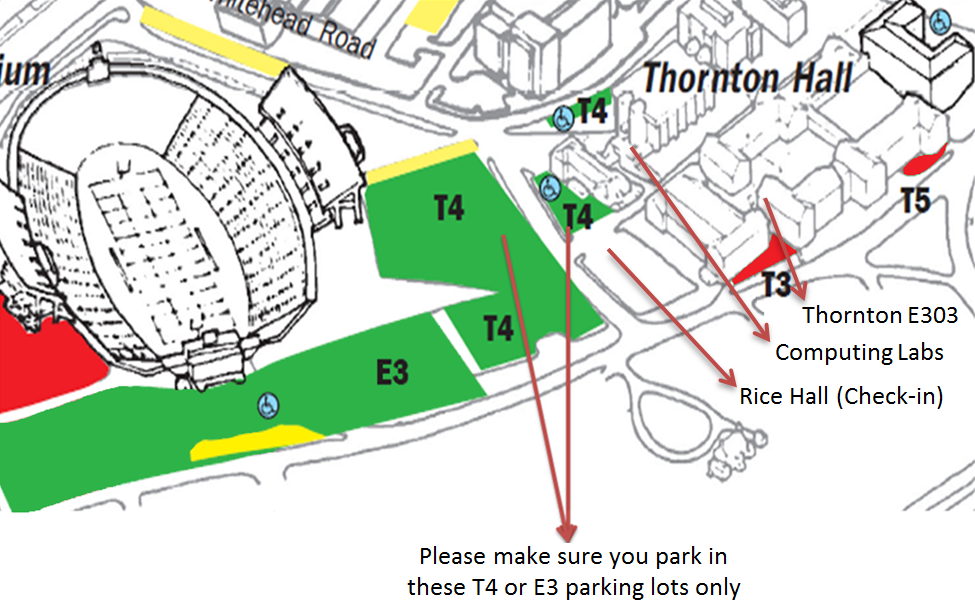
\includegraphics[width=5in]{images/HSPC-2012-Site-Map.png}
\end{center}
\end{figure}

\noindent We have all been working hard to get ready, and are really
excited; hopefully you're looking forward to the contest as much as we
are.

\noindent Regards,\newline\noindent  Jane Doe \newline\noindent
HSPC Chair


\section{Media release email request}

Email subject: ``UVa HSPC: Media Release Form''; attachment was the
Photo-Permission-Form.pdf.

\noindent Hello again teams,

\noindent We have a last minute request for you; we are trying to get
the local media to cover this weekend's event. In order for them to
include a photo and for us to publish a gallery of the event online we
need a release from everyone pictured. This is completely {\bf
optional} and will have no effect on the team on the day of the
contest, but we would appreciate it if you can get the signatures. For
contestants under the age of 18, we need a parent or legal guardian's
signature. If you are able to get the forms signed, you may turn them
in to us at registration.

\noindent Thanks,\newline\noindent  Jane Doe \newline\noindent
HSPC Chair


\end{document}
